\documentclass[12pt, draftclsnofoot, onecolumn]{IEEEtran}
\usepackage{tikz}  \usetikzlibrary{arrows,positioning,shapes.geometric, arrows} 
%\documentclass[journal,comsoc]{IEEEtran}
\setcounter{tocdepth}{2} 
\usepackage{cite}
\usepackage{amsmath,amssymb,amsfonts}
\usepackage{algorithmic}
\usepackage{graphicx}
\usepackage{float} 
\usepackage{subfigure}
\usepackage{textcomp}
\usepackage{xcolor}
%\usepackage{ctex}
\usepackage{booktabs}
\usepackage{caption}
\usepackage[colorlinks]{hyperref}
\usepackage{url}
\usepackage{graphicx}
\usepackage[T1]{fontenc}% optional T1 font encoding
% \chapter{title}
\newcommand{\etal}{\textit{et al. }}
\ifCLASSINFOpdf
  % \usepackage[pdftex]{graphicx}
  % declare the path(s) where your graphic files are
  % \graphicspath{{../pdf/}{../jpeg/}}
  % and their extensions so you won't have to specify these with
  % every instance of \includegraphics
  % \DeclareGraphicsExtensions{.pdf,.jpeg,.png}
\else
  % or other class option (dvipsone, dvipdf, if not using dvips). graphicx
  % will default to the driver specified in the system graphics.cfg if no
  % driver is specified.
  % \usepackage[dvips]{graphicx}
  % declare the path(s) where your graphic files are
  % \graphicspath{{../eps/}}
  % and their extensions so you won't have to specify these with
  % every instance of \includegraphics
  % \DeclareGraphicsExtensions{.eps}
\fi
% graphicx was written by David Carlisle and Sebastian Rahtz. It is
% required if you want graphics, photos, etc. graphicx.sty is already
% installed on most LaTeX systems. The latest version and documentation
% can be obtained at: 
% http://www.ctan.org/pkg/graphicx
% Another good source of documentation is "Using Imported Graphics in
% LaTeX2e" by Keith Reckdahl which can be found at:
% http://www.ctan.org/pkg/epslatex
%
% latex, and pdflatex in dvi mode, support graphics in encapsulated
% postscript (.eps) format. pdflatex in pdf mode supports graphics
% in .pdf, .jpeg, .png and .mps (metapost) formats. Users should ensure
% that all non-photo figures use a vector format (.eps, .pdf, .mps) and
% not a bitmapped formats (.jpeg, .png). The IEEE frowns on bitmapped formats
% which can result in "jaggedy"/blurry rendering of lines and letters as
% well as large increases in file sizes.
%
% You can find documentation about the pdfTeX application at:
% http://www.tug.org/applications/pdftex


\usepackage{amsmath}
\interdisplaylinepenalty=2500
\usepackage[cmintegrals]{newtxmath}
\hyphenation{op-tical net-works semi-conduc-tor}

\begin{document}
\tableofcontents
\title{Towards Cloud Native Satellite-Terrestrial Integrated Networks}
\author{Xiaohe~He,~\IEEEmembership{Student Member,~IEEE,}
\thanks{X. He was with the School of Information and Science Technology, ShanghaiTech University, Shanghai, 201210 China e-mail: (hithxh@gmail.com).}% <-this % stops a space
}

% The paper headers
\markboth{Journal of \LaTeX\ Class Files,~Vol.~14, No.~8, August~2015}%
{Shell \MakeLowercase{\textit{et al.}}: Bare Demo of IEEEtran.cls for IEEE Communications Society Journals}

% make the title area
\maketitle

% As a general rule, do not put math, special symbols or citations
% in the abstract or keywords.
\begin{abstract}
The upcoming 5G and beyond wireless communications are expected to higher data-rates, lower latency and support heterogeneous service scenarios. Key features of satallite communication such as wide-scale coverage, broadcast/multicast and high availability anticipate new opportunities for satallite communications services to become an integral part of terrestrial systems. Satellite-terrestrial integrated networks (STIN) can not only extend the coverage of terrestrial networks, but enhance the flexibility and data capability of satellite networks, attracting more attention form the academia and the industry. However, a unified definition of STIN has not yet been presented, and the research background and current status of STIN are not clear. Considering the emerging applications and research of STIN, in this article, we investigate existing technologies, propose an cloud-native STIN architecture. Specifically, we discuss the basic architecture and key technologies of cloud-native STIN. In addition, diversity gains and challenges are analyzed briefly. Finally, some future work is highlighted and wider applications of cloud-native STIN are provided for further research. 
\end{abstract}

% Note that keywords are not normally used for peerreview papers.
\begin{IEEEkeywords}
Satellite-Terrestrial Integrated Networks, Cloud-native, Intent-Driven Network, 5G, SDN, NFV.
\end{IEEEkeywords}
% For peer review papers, you can put extra information on the cover
% page as needed:
% \ifCLASSOPTIONpeerreview
% \begin{center} \bfseries EDICS Category: 3-BBND \end{center}
% \fi
%
% For peerreview papers, this IEEEtran command inserts a page break and
% creates the second title. It will be ignored for other modes.
\IEEEpeerreviewmaketitle
\section{Introduction}


The 5G and beyond wireless communication systems are envisioned to provide 1000-fold improvement in capability, 10-100 times higher end-user data-rates, 5 times reduced end-to-end (E2E) latency, 10 times increased energy efficiency for low-power devices and to support 10-100 times higher number of ubiquitously connected devices with diverse quality-of-service (QoS) as compared to the 4G\cite{sharma2018satellite}.

In terms of capacity and data-rate, legacy terrestrial networks have significant advances. However, due to cost and implementation issues, cellular base stations are difficult to be deployed in some geographically challenging areas like desert and ocean. While, key features of satallite communication such as wide-scale coverage, and high availability can over these deficiencies, fostering the roll-out of services in areas that cannot be covered by terrestrial networks, reinforcing massive-machine-type communications reliability by providing service continuity for fast-moving platforms, enabling network scalability by providing efficient multicast/broadcast resource for data delivery towards the clients. It also anticipate new opportunities for satallite communications services to become an integral part of terrestrial systems. \cite{sharma2018satellite} detaily discussed some key aspects satellites can play a part in the 5G network. Emerging SDN/NFV for seamless intergation of satellite and terrestrial network, and on-board processing, interference avoidance and mititgation techniques, dynamic spectrum sharing for hybrid satallite-terrestrial systems are described. 


\subsection{Satellite-Terrestrial Integrated Network} 
Integrate satellite networks and terrestrial networks will meet heterogeneous service requirements in terms of achievable coverage, data rates, latency, reliability and energy consumption, but it also present great challenges. since they were developed independently and fundamentally different.

Motivated by the above-mentioned benefits and challenges, the academia and the industry are putting significant efforts to investigating novel seamless satellite-terrestrial integrated solutions. 



Architecture

Many researches focus on Software-Defined Networking (SDN) and Network Functions
Virtualisation (NFV) based satellite-terrestrial integration scheme. 

\cite{guidotti2019architectures} discussed the architectures and the PHY/MAC procedures of 5G to incorporate satellites.


\cite{sagin} comprehensively surveyed the Space-Air-Ground Integreted Network works in network design, resource allocation, performance analysis and optimization.

\cite{zhang2017software} proposed a software defined space-air-ground integrated network architecture for supporting diverse vehicular services in a seamless, efficient, and cost-effective manner.

\cite{zhu2017non} applied non-orthogonal multiple access (NOMA) scheme to STIN, and shwoed that it can achive better user fairness and system total capacity in the downlink transmission capacity problem.

Information Centric Networking \cite{chen2020exploitation}\cite{li2019icn}



Network
\cite{liu2018space} proposed using Named Data Networking to manage the Space-Terrestrial Integrated mobility.



optimization
\cite{kato2019optimizing} Optimizing Space-Air-Ground Integrated Networks by Artificial Intelligence

There are also many schemes are proposed to optimize the hybrid satellite-terrestrial networks.


\cite{kuang2017radio} surveys the radio resource management in satellite-terrestrial networks in three main aspects: spectrum sharing, beamforming, and cross-layer power allocation.



To minimize satellite bandwidth consumption, \cite{wu2016two} introduced a two layer caching model for content delivery services in the satellite-terrestrial networks. And genetic algorithm is utilize to solve the formulated nonlinear integral programming problem .

Spectrum is an essential resource in communication systems, and how to share limited spectrum between the terrestrial and space segments is a crucial issue. \cite{jia2016broadband} applyed cognitive radio (CR) to an broadband hybrid satellite-terrestrial network to support a flexible and smart spectrum usage and management. And a cooperative spectrum sensing algorithm for mobile users of the terrestrial and space segments is proposed and demonstrated in a CR-based experimental platform using USRP and PC.

In STIN, TCP/IP architecture is not competent.
\cite{liu2018space} argured using Named Data Networking to manage the mobility of STIN. Specifically, a tracing-based producer mobility management scheme and an addressing-assisted forwarding method were proposed to optimized a Time Varing Graph modeled Multi-layered Satellite Networks. 

physical
generalized frequency division multiplexing (GFDM)
\cite{yang2018interference}\cite{yang2018data}


\cite{kodheli2017integration} consider using LEO constellation to provide backhaul connectivity to terrestrial networks. And the challenges of large delay and Doppler shifts of satallite systems for 5G PHY and MAC layer procedures are accessed. Besides, authors proposed some solutions to control the HARQ processes and UE buffer size.

































Satellite and Terrestrial Network for 5G (SaT5G)\cite{sat5g} aims to develop a cost effective “plug and play” satcom solution for 5G, and focussed on the implementation of 5G SDN \& NFV in Satellite Networks, integrated Network Management and Orchestration, multilink and Heterogeneous Transport Optimisation, harmonisation of Satcom with 5G Control and User Planes, extension of 5G Security to Satellites, caching and Multicast for Optimised Content and VNF Distribution.

SANSA project\cite{sansa} proposed a spectrum efficient STIN based on three key principles: 
\begin{itemize}
	\item A seamless integration of the satellite segment into terrestrial backhaul networks;
	\item A terrestrial wireless network capable of reconfiguring its topology according to traffic demands;
	\item A shared spectrum between satellite and terrestrial segments.
\end{itemize}

Project VITAL \cite{vital} brought NFV into satellite domain,  enabled SDN-based, federated resource management in STIN and provided a unified control plane for operators to efficiently manage and optimize the operation of STIN.

An architecture of STIN based on SDN/NFV is shown as Fig.1. SDN separates the control plane from the data plane through a well-defined programming interface, such that the centralized controller can have a complete overview of the network. While NFV decouples network functions from dedicated physical equipment, and runs the virtual network functions (VNFs) in the general purpose physical or virtual network appliances.  SDN and NFV complement each other to achive better performance. Thses paradigms enable network to be programble and makes the network more flexible, scalable, and in turn leads to agile servive deployment and lower capital and operational expenses.
\begin{figure}[H] 	
	\centering 	
	\includegraphics[width=\columnwidth]{img/stin.png} 	\caption{An architecture of STIN based on SDN/NFV} 
\end{figure}



\subsection{Cloud Native}
Cloud-native\cite{cncf} is a way to build and run applications that fully exploit the cloud computing model. Applications are composed of independent microservices and can run on a container platform, like Kubernetes. This technology increases the application flexibility, supports continuous integration and deployment (CI/CD).
\subsubsection{Microservices}
Traditionally, applications are built in monolith architecture, all processes are tightly coupled and run as a single service. If one application process sees a high demand, the architecture as a whole must be scaled. Add or improve the features of a monolithic application becomes more complicated, which makes it difficult to implement new ideas. Monolithic designs also pose a risk to applications, as numerous dependent, close-knit processes enhance the effect of the failure of a single process.

Microservices are an cloud-native architectural and organizational approach in which software is composed of small independent services that communicate over APIs. The comparation between monoliths and microservices is shown as figure 3.
\begin{figure}[H]
	\centering
	\includegraphics[width=\columnwidth]{img/microservices.png}
	\caption{ Monoliths and Microservices}
\end{figure}

Microservices architectures make applications easier to scale and faster to develop, enabling innovation and accelerating time-to-market for new features.
\subsubsection{Containers}
A container is an ready-to-run software package which contains all the requirements for running an application, including the code, runtime required for each program, application and system libraries and default settings. It decouples applications from underlying host infrastructure, making it easier to deploy applications in various different  environments (dev, test, production, etc.) or different cloud or OS settings. Container runtimes is software that responsible for running containers.

Compare to traditional virtual machines (VMs),container offer a significantly more lightweight unit for developers to work with, see Fig. 4.

\begin{figure}
	\centering
	\includegraphics[width=\columnwidth]{img/container.png}
	\caption{VM vs Container}
\end{figure}
\subsubsection{Kubernetes}
Kubernetes\cite{k8s}, also known as K8s, is an open source container orchestration engine for automating deployment, scaling, and management of containerized applications. It groups containers that make up an application into logical units for easy management and discovery. Actually, Kubernetes is the de facto standard for container orchestration systems. It is also a kind of IDN system, expressing intents to network through YAML files.

It has many benifit features:
\begin{itemize}
	\item Automated deployment: When the application is deployed into the container, the container that runs the application in the cluster is automatically programmed by Kubernetes according to the applications computing resource requirements and other constraints. The availability of the application is not affected throughout this procedure.
	\item Self-healing: When some containers in the Kubernetes cluster fail, they will be restarted.  When some Nodes hang up, Kubernetes will automatically reschedule the containers on these Nodes to other available Nodes.  If some containers do not meet the user-defined health check conditions, these containers will be judged as not working properly, and the cluster will automatically kill these containers. In this process, the containers will not be restarted or rescheduled until they are available.
	\item Horizontal scaling: In Kubernetes, the horizontal scaling of the application can be achieved with a single command, the HPA (Horizontal Pod Autoscaler).  HPA is implemented through Kubernetes API Resource and Controller, where Resource determines the behavior of Controller, and Controller periodically adjusts the number of replicas in Replication Controller or Deployment, so that the observed average CPU usage can match the user-defined.
	\item Service discovery and load balancing:  Kubernetes has a built-in service discovery function. It assigns an IP address to each container and assigns a DNS name to a group of containers. Through this, the load balancing function of the service can be realized.
	\item Automatic update and rollback: When the application we develop changes, Kubernetes can implement rolling updates while monitoring the status of the application to ensure that all instances will not be killed at the same time, causing the application to be unavailable for a period of time.  If an application update fails at some point, Kubernetes can automatically restore the application to its original correct state.
\end{itemize}

\subsubsection{Service mesh} 
[cite https://istio.io/latest/about/service-mesh/]
Modern applications are typically architected as distributed collections of microservices, with each collection of microservices performing some discrete business function. A service mesh is a dedicated infrastructure layer that you can add to your applications. It allows you to transparently add capabilities like observability, traffic management, and security, without adding them to your own code. The term “service mesh” describes both the type of software you use to implement this pattern, and the security or network domain that is created when you use that software.

As the deployment of distributed services, such as in a Kubernetes-based system, grows in size and complexity, it can become harder to understand and manage. Its requirements can include discovery, load balancing, failure recovery, metrics, and monitoring. A service mesh also often addresses more complex operational requirements, like A/B testing, canary deployments, rate limiting, access control, encryption, and end-to-end authentication.

Service-to-service communication is what makes a distributed application possible. Routing this communication, both within and across application clusters, becomes increasingly complex as the number of services grow. Istio helps reduce this complexity while easing the strain on development teams

Istio is an open source service mesh that layers transparently onto existing distributed applications. Istio’s powerful features provide a uniform and more efficient way to secure, connect, and monitor services. Istio is the path to load balancing, service-to-service authentication, and monitoring – with few or no service code changes. Its powerful control plane brings vital features, including:  Secure service-to-service communication in a cluster with TLS encryption, strong identity-based authentication and authorization Automatic load balancing for HTTP, gRPC, WebSocket, and TCP traffic Fine-grained control of traffic behavior with rich routing rules, retries, failovers, and fault injection A pluggable policy layer and configuration API supporting access controls, rate limits and quotas Automatic metrics, logs, and traces for all traffic within a cluster, including cluster ingress and egress.
\begin{figure}[H]
	\centering
	\includegraphics[width=\columnwidth]{img/istio.png}
	\caption{Istio architecture}
\end{figure}
Istio has two components: the data plane and the control plane.

The data plane is the communication between services. Without a service mesh, the network doesn’t understand the traffic being sent over, and can’t make any decisions based on what type of traffic it is, or who it is from or to.

Service mesh uses a proxy to intercept all your network traffic, allowing a broad set of application-aware features based on configuration you set.

An Envoy proxy is deployed along with each service that you start in your cluster, or runs alongside services running on VMs.

The control plane takes your desired configuration, and its view of the services, and dynamically programs the proxy servers, updating them as the rules or the environment changes.
 
\subsubsection{CI/CD}
Software development raises the demand for automation throughout the phases of build, test, and release, particularly when software is being developed rapidly and efficiently. Thus, the CI/CD(continuous integration and deployment) technique comes into being. It has three different stages:
\begin{itemize}
	\item Continuous integration: The ability to frequently merge changes back into the master branch, validate changes via build creation, and run automated tests. Integrating modifications into the release branch in advance can lower integration effort during software release.
	\item Continuous delivery: An expansion of continuous integration to make software updates quick and sustainable. Automated testing on top of automated release process and simple software deployment allows for flexible release plans and easy troubleshooting by deploying smaller release batches to production early.
	\item Continuous deployment: This is a level above continuous delivery. Changes that have passed through all pipeline stages are distributed to the consumer. There is no human interference. Only failing tests block the deployment of new changes.
\end{itemize}

The CI/CD pipeline ensures that automation takes over the integration, delivery, and deployment process. It not only allow agile development of applications, but bring faster time to market.

\section{Cloud native STIN}
Fortunately, a ray of hope comes shining telecom providers’ way with the new progress and achievements in the Artificial Intelligence (AI), cloud computing, and micro-services era. 

\subsection{Architecture}
The architecture of STIN is shown as Fig. 5. It is very similar to Service-Based-Architecture (SBA) of traditional terrestrial 5G networks\cite{3gpp.23.501}, but has an modification in RAN to support satellite networks.
\begin{figure}[H]     
	\centering     
	\resizebox{\textwidth}{!}{%
		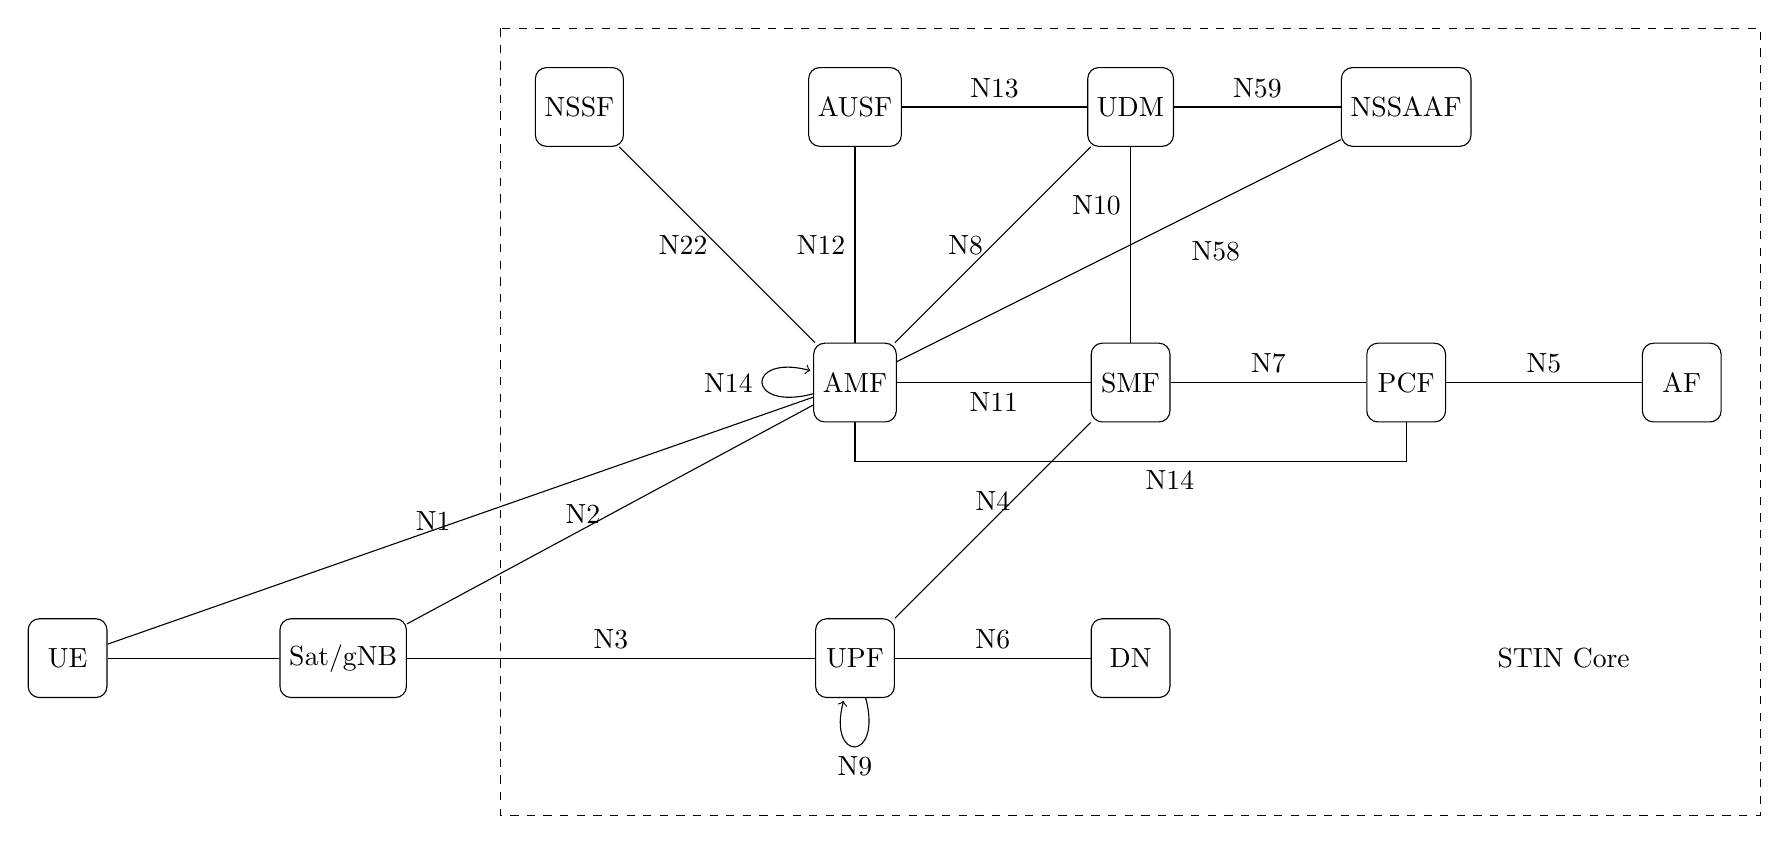
\begin{tikzpicture}[-,node distance=2.5cm,auto,main node/.style={rectangle, minimum width=1cm, minimum height=1cm,rounded corners,draw,align=center}] 
		%定义流程图具体形状  
		\node [main node](NSSF)  {NSSF};  
		\node [main node](AUSF) [right of = NSSF, xshift = 1cm] {AUSF};   
		\node [main node](UDM) [right of = AUSF, xshift = 1cm] {UDM};    
		\node [main node](NSSAAF) [right of = UDM, xshift = 1cm] {NSSAAF};   
		\node [main node](AMF) [below of = AUSF,yshift = -1cm] {AMF};    
		\node [main node](SMF) [ right of = AMF, xshift = 1cm] {SMF};    
		\node [main node](PCF) [right of = SMF, xshift = 1cm] {PCF};     
		\node [main node](AF) [right of = PCF, xshift = 1cm] {AF};     
		\node [main node](UPF) [ below of = AMF, yshift = -1cm] {UPF};   
		\node [main node](RAN) [left of = UPF, xshift = -4cm] {Sat/gNB};     
		\node [main node](UE) [left of = RAN, xshift = -1cm] {UE};      
		\node [main node](DN) [right of = UPF, xshift = 1cm] {DN};     		
		\node (caption) [thick, right of = DN, xshift = 3cm] {STIN Core};   

		\draw (PCF) --++(0,-1) -| node [xshift = 4cm, below]{N14}(AMF);     
		\path 
		(NSSF) edge node [left]{N22} (AMF) 
		(AUSF) edge node [left]{N12} (AMF) 
		(UDM) edge node [left]{N8}(AMF) 
		(NSSAAF) edge node [xshift = 0.8cm,right]{N58}(AMF) 
		(AUSF) edge node [above]{N13}(UDM) 
		(UDM) edge node [above]{N59}(NSSAAF)  
		(UDM) edge node [yshift = 0.5cm, left]{N10}(SMF)  
		(AMF) edge node [below]{N11}(SMF)   
		(SMF) edge node [above]{N7}(PCF)  
		(PCF) edge node [above]{N5}(AF)  
		(UE) edge node [left]{N1}(AMF) 
		(UE) edge (RAN) 
		(RAN) edge node [left]{N2}(AMF)    
		(RAN) edge node [above]{N3}(UPF)    
		(UPF) edge node [above]{N6}(DN)    
		(UPF) edge node [above]{N4}(SMF) 
		(AMF) edge [loop left] node [left]{N14}(AMF) 
		(UPF) edge [loop below] node [below]{N9}(UPF); 
		\draw [dashed](-1,1) rectangle (15,-9);  
		\end{tikzpicture}
		}%     
	\caption{Architecture of cloud native STIN}   
\end{figure}
\subsection{Core}

The major network functions and entities  of 5G core are listed below:
\begin{itemize}
	\item AMF (Access and Mobility management Function): Manages access control and mobility.
	\item SMF (Session Management Function): Set up and manage sessions based on network policy.
	\item UPF (User Plane Function): Can be deployed in various configurations and locations based on the service type.
	\item PCF (Policy Control Function ): Provides a policy framework incorporating network slicing, roaming and mobility management.
	\item UDM (Unified Data Management): Stores subscriber data and profiles.
	\item AUSF (Authentication Service Function): An authentication server as the name implies.
	\item NSSF (Network Slicing Selection Function): Can be used by the AMF to assist the selection of the Network Slice instances that will serve a particular scenario and to allocate an appropriate AMF if the current one is not able to support all network slice instances for given device.
\end{itemize}

It uses service-based interfaces to connect control-plane functions and user-plane functions are connected by point-to-point links. This architecture and standardized  interfaces that can be deployed on  a shared, orchestrated cloud infrastructure, that is cloud-native STIN.

There are many projects works on applying cloud native scheme to terrestrial 5GC. 
In the industry, componies like SAMSUNG\cite{samsung}, Ericsson\cite{ericsson}, ZTE\cite{zte}, Oracle\cite{oracle} released their cloud-native 5GC solutions, moving their 5GC network as well as crucial network functions for new industry solutions to the cloud.


In academia, many researches did impressive work in this field. 

In \cite{arouk20205g}, authors deployed an cloud-native 5G demo based on K8s and Openshift Operator. And demonstrated the automation and auto-configuration of this network. 

In \cite{arouk2020kube5g}, authors proposed a cloud-native 5G service platform - Kube5G. It introduces a novel approach in building and packaging a cloud-native compliant telco network function (NF) in a form of nested well-defined layers and present a workflow for CI/CD operations in support of multi-version network functions (physical, virtual and cloud functions).

\cite{dab2020cloud} \cite{dab2020efficient} introduced a cloud-native service function chaining framework and proposed an optimized network-aware load balancing algorithm capable of carrying efficiently the traffic while considering the underlying infrastructure network state.

\cite{du2020cloud} develop a cloud-native based implementation of Access and Mobility Management Function (AMF) under the OAI 5G Core project and the AMF is tested in a real E2E 5G system for its functionalities. Also, it's deployed in a cloud environment, tested with simulated gNB/UEs, for its stability and concurrency capacity.

Apart from most researches focused on 5GC, \cite{balasubramanian2021ric} focused on intelligent cloud-native RAN. It disaggregated the traditional monolithic RAN into adio antenna unit situated at the cell tower, the 5G base station distributed unit (DU) and the control unit (CU) at the edge cloud. Disaggregation of the CP and UP, the RAN is more flexible and allows for independent scaling. Besides, it can also improve customer experience by using machine learning/ deep learning (ML/DL)-driven policies to tailor the RAN for unique spectrum position and geography based on a holistic area-wide network view. 


For 5g network slicing, \cite{sharma2017cloud} presents a cloud-native approach to network slicing framework, which covers the entire life cycle of network slices, encompassing their design, creation, deployment, customization, and optimization. And a proof-of-concept implementation is described to demonstrates its key principles. 

Free5GC \cite{free5gc} and UERANSIM\cite{ueransim} are two popular simulation tool for 5G core and ue/ran. And can be deployed in the cloud to demonstrate the 5G scenarios.

\subsection{RAN}
RAN is the most essential part of STIN, it provides wide-area wireless connectivity to mobile devices.

However, since the different develop route, it 
\subsubsection{SD-RAN}


3GPP architected the RAN using a protocol stack. To provide more flexibility, RAN can be further disaggregated in three-tiers across two dimensions. 

The first level is the horizontal division, which essentially divides the RAN protocol, allowing the various components to be separately produced. This addresses the issues of high owning costs, high energy consumption, improved system performance through intelligent and dynamic radio resource management, open innovation in many components, while assuring multi-vendor operation.

The second tier of disaggregation is vertical, focusing on control/user plane separation (CUPS) of the CU, further disaggregating it into CU-U, the logical node hosting the user-plane part of the PDCP protocol and SDAP protocol, and CU-C, the logical node hosting the control-plane part of the PDCP protocol and the RRC protocol.

The third-tier of disaggregation follows the SDN paradigm by carrying vertical disaggregation one step further. It dose this by separating most of RAN control (RRM functions) from the disaggregated RAN components (mainly from CU-C), and logically centralizing them as applications running on an SDN controller, which is labelled as the near real-time RAN Intelligent controller (nRT-RIC) In the O-RAN Architecture.

3GPP defined numbers of horizontal disaggregation options. 
\begin{figure}
	\includegraphics[width=\columnwidth]{img/ran.png}
	\caption{3GPP specified RAN disaggregation options}
\end{figure}

\cite{checko2014cloud} gave an overview of cloud RAN.

O-RAN\cite{oran} is a disaggregated, open, virtualized, and intelligent RAN reference architecture under development


Consistent with O-RAN, ONF proposed a cloud-native  \cite{sunay2020onf}










Insprired by the ideas above, we propose one novel architecture for satellite-terrestrial integrated network on the ground of cloud native, suggesting new ideas of the integration of satellite netoworks and terrestrial networks. Armed by powerful functions of cloud computing, the cloud-native STIN can provide more flexible resource scheduling, traffic management and network scalability. The architecture is shown as below.


\begin{figure}[H]
	\centering
	\includegraphics[width=\columnwidth]{./img/cnstin.png}
	\caption{Proposed architecture of cloud-native STIN}
\end{figure}


Robust test framework and validation facilities is important to reduce potential flaws in the user applications that will be uploaded to the satellite.
The user connects to the test and simulation infrastructure through a computer to write code, and then after successful debugging, the test is no problem, and it is sent to the shared satellite through the ground station for operation.

Although the pay-as-you-go cost of having saas satellite as a service is much lower than the cost of launching a satellite by itself, it is still very expensive. Although it is not as expensive as ASICs, it is better to be like super computing when debugging the software on the satellite.  As with running programs, it is best to reduce the time to debug bugs on the computer.  Therefore, there must be a testing software framework on the ground to ensure the quality of the satellite software.  The mechanism of continuous integration and continuous release, and the satellite digital twin hardware test environment on the ground.
\begin{figure}
	\centering
	\includegraphics[width=\columnwidth]{img/missiondesign.png}
	\caption{Mission design}
\end{figure}


The user code first goes through the CI/CD process to generate the deployment program, and then it is put on the basic hardware verification platform to run smoke test to ensure the normal basic function, and then it is run on the satellite digital twin hardware verification platform. After passing, it is released to the satellite mission control center, where it is deployed and run on the satellite.
\begin{figure}[H]
	\centering
	\includegraphics[width=\columnwidth]{img/cicd.png}
	\caption{CI/CD framework}
\end{figure}


In order to prevent third-party software from destroying the hardware (waste satellite's precious battery, point the optical sensor at the sun, or randomly control the satellite's attitude, etc.), an intermediate command layer is also needed to prevent these potential risks caused by user code.  In addition, a monitoring software is required to monitor the operation of the user's program, and the user's program will be stopped at critical moments.  The satellite operator of the ground station, in the event of an accident, can manually stop the user's program remotely.  Use segments to ensure the security of user code.  The satellite communication bus allows the user code to control the mission load, ground station communication, attitude control and satellite power control.  The most important aspect of the software framework is security.

\begin{figure}
	\centering
	\includegraphics[width=\columnwidth]{img/security.png}
	\caption{satellite as a service security}
\end{figure}












\subsubsection{Satellite as a service}
Modern space industry is witnessing an exponential growth of micro satellites, with the numbers of successfully launched went from single digits annually in the years before 2008 to hundreds now\cite{nanosates}.

\begin{figure}[H]
	\centering
	\includegraphics[width=\columnwidth]{./img/microsate.png}
	\caption{Nanosatellite launches}
\end{figure}

A shared-access, single host/multi-tenant satellite platform can offer an ability to host multiple missions  on a single spacecraft, sharing the capabilities of both platform and payload instruments between multiple customers that can perform mission operations according to their needs. It can dramatically lower the cost and accelerate the development of space technology.

Satellite as a service\cite{saas} enables people to control satellite communications, process satellite data, and scale the satellite operations without having to build  or manage their own satellite infrastructures.



Key features of satellite communications such  as  wide-scale coverage, broadcast/multicast support, anticipate new opportunities for satellite communications services to be integrated with terrestrial networks.

However, to materialize these opportunities, satellite      communications services have to be provisioned and  operated in a more flexible, agile and cost-effective manner. 









In this section, we describe solutions for   the virtualization of satellite  ground segment that builds on Software Defined Networking (SDN) and Network Function Virtualization (NFV) technologies.


AWS Ground Station \cite{AWS} is a fully managed service provided by Amazon that enables people to control satellite communications,process satellite data, and scale the satellite operations.  Users don't have to build or manage their own ground station infrastructure. 

Amazon also works with satellite operators like Iridium Communications to offer its Iridium CloudConnect IoT service.

iridium work with AWS provide  a satellite cloud-based adapter service CloudConnect, it transfers Short Burst Data (SBD) messages from iridium-connected devices to the AWS cloud. 

\begin{figure}[H]
	\centering
	\includegraphics[width=5 in]{./img/iridium.png}
	\caption{Iridium CloudConnect SBD on AWS }

\end{figure}



Microsoft's Azure Orbital \cite{Azure} is another Ground Station As-a-Service (GSaaS) that provides communication and control of satellites. It enables customers to communicate, downlink, and process data from satellites/spacecrafts on a pay-as-you-go basis without needing people to build their own satellite ground stations. With Azure Orbital, data can be ingested into Azure directly, which enables seamless application and use of cloud services such as compute, storage, AI, and data analysis for fast data processing. 

Besides, Microsoft has teamed up with SpaceX and SES to launch Azure Space\cite{Azurespace} to bring cloud computing to space. Working with a number of industry leaders like SpaceX, SES, KSAT, Viasat, Kratos, AMEGINT, KubOS  and US Electrodynamics, Azure Space aims to make space connectivity and compute increasingly attainable across industries including agriculture, energy, telecommunication, and government.


Azure Space will support O3B Medium Earth Orbit (MEO) constellation and provide high-speed, low-latency satellite broadband for Azure Modular Datacenter (MDC) through SpaceX Starlink.



With AWS Ground Station, we can now achieve Automated Earth observation\cite{eos}
\begin{figure}[H]
	\centering
	\includegraphics[width=\columnwidth]{img/eos.png}
	\caption{Automated AWS Ground Station EOS}
\end{figure}
\begin{enumerate}
	\item During a satellite contact, the AWS Ground Station Amazon S3 data delivery services deposit the downlink data as VITA 49 in .pcap files in an S3 bucket.
	\item When AWS Ground Station has finished writing all .pcap files it generates an Amazon CloudWatch event.
	\item The CloudWatch event triggers an AWS Lambda function.
	\item The Lambda function strips out the payload data from the .pcap files into .bin raw data files. Then starts the RT-STPS processor EC2 instance.
	\item The RT-STPS EC2 instance combines the raw data into a single file, which it then processes into level 0 data using RT-STPS.
	\item The RT-STPS EC2 instance pushes the data to S3, sends an Amazon Simple Notification Service (Amazon SNS) notification, then shuts down.
	\item The Amazon SNS notification triggers a Lambda function, which starts up the processor EC2 instance.
	\item The IPOPP EC2 instance pulls the data from S3, then processes it using IPOPP.
	\item The IPOPP EC2 instance pushes the Level 1A, Level 1B, and Level 2 data it produces to S3.
	\item The IPOPP EC2 instance sends an SNS notification then shuts down.
	
\end{enumerate}







Horizontal analytics
RAN
Core



\subsection{OAI}
OpenAirInterface (OAI)\cite{OAI} is an open-source project that implement the 3GPP technoligy on general prupose x86 computing hardware and Off-The-Shelf (COTS) Software Defined Radio (SDR) cards like the Universal Software Radio Peripheral (USRP).

Many researches use OAI to deploy 4G solutions\cite{nikaein2014openairinterface}\cite{powder}\cite{chun2016performance}. Now, OAI are working on the open-source 5G Next Radio(NR) and 5G Core Network(5GC)\cite{kaltenberger2020openairinterface} and satellite scenarios.

\cite{imadali2018cloud} briefly reviewed the design principles of cloud-native 5G VNF, paving a way to new era of intelligent 5G in OAI community.

Authors in \cite{kaltenberger2019openairinterface} described a fully standard compliant implementation of 5G NR that is inter-operable with commercial equipment.


\cite{du2020cloud} developed a minimum cloud-native Access and Mobility Management Function (AMF) of 5GC. And they also built an E2E 5G SA system using their own SMF and UPF and commercial Huawei CPE, Amari soft gNB to verify the AMF’s functionalities. However, its current AMF still not support some important functions, such as handover, mobility registration, roaming, etc.


\cite{arouk20205g} presented a cloud-natiove demo on 5G dynamic automation and management using Openshift operator Kube5G\cite{arouk2020kube5g}. Some important principles of 5G, like change of network configuration, network entities upgrade, switch between monolithic RAN and disaggregated RAN were demonstrated. It shows that 4G/5G network can be provisioned in less than two minutes, and updated/reconfigured in less than a minute. 

Apart from terrestrial developments in OAI, researchers also trying to extend 5G NR slolutions to satellite networks.

Based on the important 5G protocol stack implementation of \cite{allstar}\cite{champion}, Fraunhofer IIS contributed to OAI with selected features of the 5G NR waveform and the adaptations for satellite communication. And following 3GPP Work Item on Non-Terrestrial-Networks\cite{811}\cite{821}, 5G-GOA\cite{GOA}, which was mostly contributed by Fraunhofer IIS and the Munich Center for Space Communications (Bundeswehr University Munich), extended the 5G New Radio standard to enable direct radio access of terrestrial communication networks via satellites. It used an emulator, and also live, over the air demonstration\cite{kaltenbergerbuilding} to test and verify the performance. Both 5G gNB and UE are based on software-defined OAI. 


\section{Challenges}
\subsection{Benifits}
\subsection{Network Management}
\subsubsection{Resource Allocation}
\cite{boudi2021ai} proposed an Artificial Intelligence based Resource aware Orchestration (AIRO) framework for 5G based on ETSI Zero-touch network and Service Management concept (ZSM), cloud-native approach and Machine Learning (ML) solutions. Further, a simulation platform has been introduced to verify the efficiency of a cloud-native cluster. 

Traffic steering and load balancing of cloud-native 5G is essential. Boutheina Dab \textit{et al.} designed and deployed an cloud-native 5G service function chaining architecture based on network service mesh\cite{NSM} and Kubernetes. Besides, two traffic steering scheme NA-TS\cite{dab2020efficient} and MG-NLB\cite{dab2020cloud}, which were based on Weighted Round Robin and Maglev\cite{eisenbud2016maglev} respectively, were deployed to optimize network performance.


\subsubsection{Network slicing}
\cite{sharma2017cloud} built an proof-of-concept system that runs on a complete end-to-end 5G network, and firsly deployed cloud-native approach to create, orchestrae, and optimize network slices.


\section{Cloud native security}
Cloud native application development promises agility and scability, but also poses some special security challenges. Cloud native security mainly consider four layers: Cloud, Clusters, Containers, and Code\cite{security}. In each layer, there are security related concerns.

\subsection{Container security}
container escape, a container is run with excessive privileges or punches holes through the security protection offered by kernel capabilities, will make other containers even the host machine itself at serious risk. it is possible to “break out” of a host’s relatively standard security controls includes the following:

Disrupting services on any or all containers on the host, causing outages
■ Attacking the underlying host to cause a denial of service by causing a stress event with a view to exhaust available resources, whether that be RAM, CPU, disk space capacity, or I/O, for example
■ Deleting data on any locally mounting volumes directly on the host machine or wiping critical host directories that cause system failure
■ Embedding processes on a host that may act as a form of advanced persistent threat (APT), which could lie dormant for a period of time before being taken advantage of at a later date

To get rid of this kind of problem, Some container conpanies like Docker and Podman provide rootless model to harden the containers. Specifically, they use an extended feature "user namespaces" to effectively fool a container into thinking that it was using a host’s user ID (UID) and group ID (GID) normally, However, from a host’s perspective the UID/GID used in the container was being run without any privileges and so was of much less consequence to the host’s security.

For container runtime security, opensource falco and commercial tools Prisma Cloud Compute Edition and Aqua from AquaSec could offer some support. 





\subsection{Orchestrator security}
Kubernetes 
To test container orchestration platforms like k8s, we could use kube-hunter. 

- authorization
- network hardening
- workload hardending


\subsection{DevSecOps}
CI/CD 

git repository 

\subsection{Cloud Platform security}
- storage
- cloud auditing 




\subsection{Container Network Interface}
https://itnext.io/benchmark-results-of-kubernetes-network-plugins-cni-over-10gbit-s-network-updated-august-2020-6e1b757b9e49

\begin{table}
	
\end{table}
Flannel
Calico 
Cilium
Weave




\cite{mendki2021securing} introduced some possible solutions for network security, container security, identity management and authentication and audit log with blockchain.


\section{Conclusion}



\ifCLASSOPTIONcaptionsoff
  \newpage
\fi

\bibliography{reference}{}
\bibliographystyle{IEEEtran}

\begin{IEEEbiography}[{\includegraphics[width=1in,height=1.25in,clip,keepaspectratio]{./img/hithxh.jpg}}]{Xiaohe He}
received his Bachelor of Science (B.Sc), in field of electronics and information engineering, from Harbin Institute of Technology (Weihai), China, in 2015. Then he joined the Schoool of Information Science and Technology, ShanghaiTech University to continue his study to Doctor of Philosophy (PhD), in 2017. 
His research interests lie in the integration of SDN/NFV based satellite and terrestrial networks.
\end{IEEEbiography}


\end{document}